\documentclass[twocolumn, amsmath, amsfonts, amssymb, trackchanges]{aastex62}
\usepackage{mathtools}
\usepackage{natbib}
\usepackage{bm}
\newcommand{\vdag}{(v)^\dagger}
\newcommand\aastex{AAS\TeX}
\newcommand\latex{La\TeX}


\newcommand{\Div}[1]{\ensuremath{\nabla\cdot\left( #1\right)}}
\newcommand{\DivU}{\ensuremath{\nabla\cdot\bm{u}}}
\newcommand{\angles}[1]{\ensuremath{\left\langle #1 \right\rangle}}
\newcommand{\td}[1]{\ensuremath{\widetilde{#1}}}
\newcommand{\KSstat}[1]{\ensuremath{\overline{\text{KS}(#1)}}}
\newcommand{\grad}{\ensuremath{\nabla}}
\newcommand{\RB}{Rayleigh-B\'{e}nard }
\newcommand{\stressT}{\ensuremath{\bm{\bar{\bar{\Pi}}}}}
\newcommand{\lilstressT}{\ensuremath{\bm{\bar{\bar{\sigma}}}}}
\newcommand{\nrho}{\ensuremath{n_{\rho}}}
\newcommand{\approptoinn}[2]{\mathrel{\vcenter{
	\offinterlineskip\halign{\hfil$##$\cr
	#1\propto\cr\noalign{\kern2pt}#1\sim\cr\noalign{\kern-2pt}}}}}

\newcommand{\appropto}{\mathpalette\approptoinn\relax}
\newcommand{\pro}{\ensuremath{\text{Ro}_{\text{p}}}}
\newcommand{\con}{\ensuremath{\text{Ro}_{\text{c}}}}

\usepackage{color}
\newcommand{\gv}[1]{{\color{blue} #1}}

%% Tells LaTeX to search for image files in the 
%% current directory as well as in the figures/ folder.
\graphicspath{{./}{figs/}{../tex/figs/}}


\received{\today}
\revised{??}
\accepted{??}%\today}
\submitjournal{ApJ}

%%%%%%%%%%%%%%%%%%%%%%%%%%%%%%%%%%%%%%%%%%%%%%%%%%%%%%%%%%%%%%%%%%%%%%%%%%%%%%%
%% TITLE & AUTHORS
\shorttitle{Stratified Thermals}
\shortauthors{Anders et al.}

\begin{document}
\title{Entrainment of low Mach number thermals in stratified domains}

\correspondingauthor{Evan H. Anders}
\email{evan.anders@colorado.edu}

\author[0000-0002-3433-4733]{Evan H. Anders}
\affil{Dept. Astrophysical \& Planetary Sciences, University of Colorado -- Boulder, Boulder, CO 80309, USA}
\affil{Laboratory for Atmospheric and Space Physics, Boulder, CO 80303, USA}
\author[0000-0002-7635-9728]{Daniel Lecoanet}
\affil{Princeton Center for Theoretical Science, Princeton, NJ 08544, USA}
\affil{Department of Astrophysical Sciences, Princeton, NJ 08544, USA}
\author[0000-0001-8935-219X]{Benjamin P. Brown}
\affil{Dept. Astrophysical \& Planetary Sciences, University of Colorado -- Boulder, Boulder, CO 80309, USA}
\affil{Laboratory for Atmospheric and Space Physics, Boulder, CO 80303, USA}


\begin{abstract}
\end{abstract}

\keywords{hydrodynamics --- turbulence --- entrainment}

%%%%% Body of the paper
%%%%%%%%%%%%%%%%%%%%%%%%%%%%%%%%%%%%%%%%%%%%%%%%%%%%%%%%%%%%%%%%%%%%%
%% INTRODUCTION
\section{Introduction}
\label{sec:intro}
Recent observations of solar convection have revealed a convective conundrum.
Power spectra have revealed weaker flows than anticipated at large length scales
\citep{hanasoge&all2012, greer&all2015},
calling into question the existence of so-called ``giant cells'' driven by deep
convection which would manifest as powerful, large-scale motions at the solar
surface. This discrepancy between theory and observations has called into question
our fundamental understanding of convection, sparking numerous targeted investigations
the nature of convection in the Sun 
\citep{featherstone&hindman2016, omara&all2016, cossette&rast2016, kapyla&all2017,
hotta2017}.

\cite{spruit1997} hypothesized that convective motions may be driven entirely by
cool downflows at the surface of the Sun, and \citet{brandenburg2016} expanded
upon this ``entropy rain'' hypothesis. Brandenburg's work includes a careful
expansion of mixing length theory to incorporate flux contributions from nonlocal
convective motions, and handles this theory in a horizontally-averaged sense.
He includes some discussion of possible flow morphologies which could be manifestations
of this entropy rain, and even includes some brief simulations of propogating
Hill vortices. However, these simulations and discussions did not include 
include a fundamental piece of entropy rain: it is buoyant, and has an entropy
deviation from the background atmosphere.

If entropy rain does evolve into downward propagating buoyant vortex rings, it is
important to understand how buoyancy effects the filling factor of these basic
convective elements. In the context of Earth's atmosphere, so-called ``thermals''
are thought to be the nucleus of cloud formation. Thermals are buoyant areas
of fluid which evolve into propagating buoyant vortex rings, and their
evolution in the Boussinesq limit have been well studied in the laboratory
for decades \citep[see e.g.][]{morton&all1956, scorer1957}, 
and more recently have been studied through
Direct Numerical Simulation (DNS) in the laminar and turbulent regime
\citep{lecoanet&jeevanjee2018}. One fundamental result of these studies of
thermals is that they experience a large degree of entrainment: their size expands
with height and their propagation velocity slows despite their buoyant nature.
However, we do not know of a study in which the propagation of these thermals,
and thus the nature of their entrainment, is affected by a 
significant atmospheric stratification.

\begin{figure}[t!]
    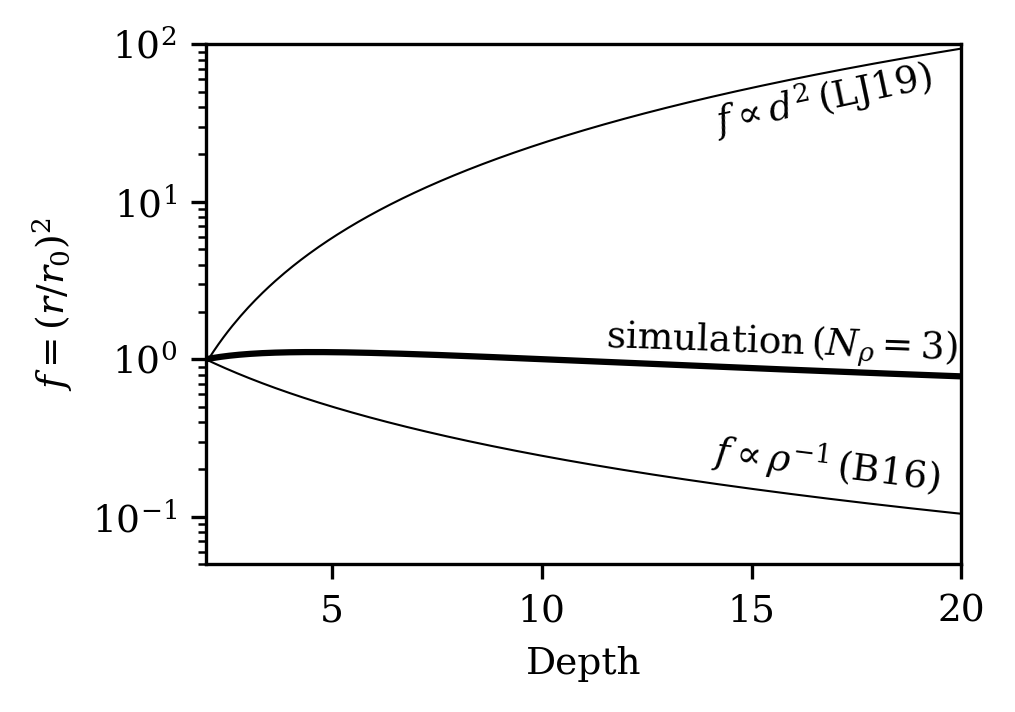
\includegraphics[width=\columnwidth]{overview_fig.png}
    \caption{We have plotted the evolution of the filling factor, or radius
	squared, of a buoyant vortex ring with depth (the $n_\rho = 3$ case examined
	later in this work). Overplotted in a thin
	solid line is the prediction for filling factor growth in the Boussinesq
	case, and in the thin dashed line is plotted the prediction for pure horizontal
	compression, as in \citet{brandenburg2016}.
    \label{fig:overview} }
\end{figure}

In the absence of buoyantly-induced entrainment, \citet{brandenburg2016}
suggests that the filling factor, $f$, of vortex rings should decrease like
$f \propto \rho^{-1}$ for horizontal compression and $f \propto \rho^{-2/3}$ for 
spherical compression. On the other hand, the filling factor of Boussinesq
thermals \emph{increases} like $f \propto d^2$, where $d$ is the depth propagated.
These regimes are shown in Fig.~\ref{fig:overview}, and compared to the true
propagation of a thermal in an appreciably stratified environment.

In this work, we extend the study of \citet{lecoanet&jeevanjee2018} to study
the propagation of low-Mach number, cold thermals in stratified domains. We are
specifically interested in how
buoyant entrainment affects the scaling of the thermal radius, or filling factor, with depth. If
buoyant entrainment is a dominant effect, it is possible that entropy rain
would simply grow too large and stall before reaching the bottom of the solar convection zone.
On the other hand, if the compression effects suggested by \citet{brandenburg2016} are the
dominant effect, then it is possible that these thermals could propagate to the bottom of the solar
convection zone, or potentially shrink to a sufficiently small size where thermal dissipation is
significant.

In section \ref{sec:theory}, we develop a theoretical description
of thermals in a stratified domain. In section \ref{sec:experiment}, we describe 
the experiments conducted in this work. In section \ref{sec:results}, we compare the results
of our experiments to the theory developed in section \ref{sec:theory}. Finally, in section
\ref{sec:discussion}, we discuss what our results imply for the entropy rain hypothesis.

%%%%%%%%%%%%%%%%%%%%%%%%%%%%%%%%%%%%%%%%%%%%%%%%%%%%%%%%%%%%%%%%%%%%%%%%%%%%%%
%% THEORY SECTION
\section{Theory}
\label{sec:theory}

\subsection{Phenomenological description of thermal evolution}
We show pictorally the evolution of a cold thermal from rest in 
Fig.~\ref{fig:evolution_colormeshes}. In Fig.~\ref{fig:evolution_colormeshes}a,
the evolution of a thermal in a weakly stratified domain with
$n_\rho = 0.5$ density scale heights is shown. In Fig.~\ref{fig:evolution_colormeshes}b,
the evolution of a thermal in an appreciably stratified domain with
$n_\rho = 3$ density scale heights is shown. While the initial conditions are
identical in both domains (spherical specific entropy perturbations of the
same magnitude whose diameters are 5\% of the domain depth), and while in both cases
the thermal quickly evolves into a propagating buoyant vortex ring, we find that the
$n_\rho = 0.5$ case entrains and grows with depth, similarly to the Boussinesq regime.
On the other hand, the $n_\rho = 3$ case has a radius which remains approximately constant
over time, and it reaches the bottom of the domain in many fewer nondimensional freefall
time units.

In the following sections, we will use a description of the impulse and momentum of these
thermals, as determined by their buoyant nature, to describe the evolution of their depth
and radii with time.

\begin{figure}[t!]
    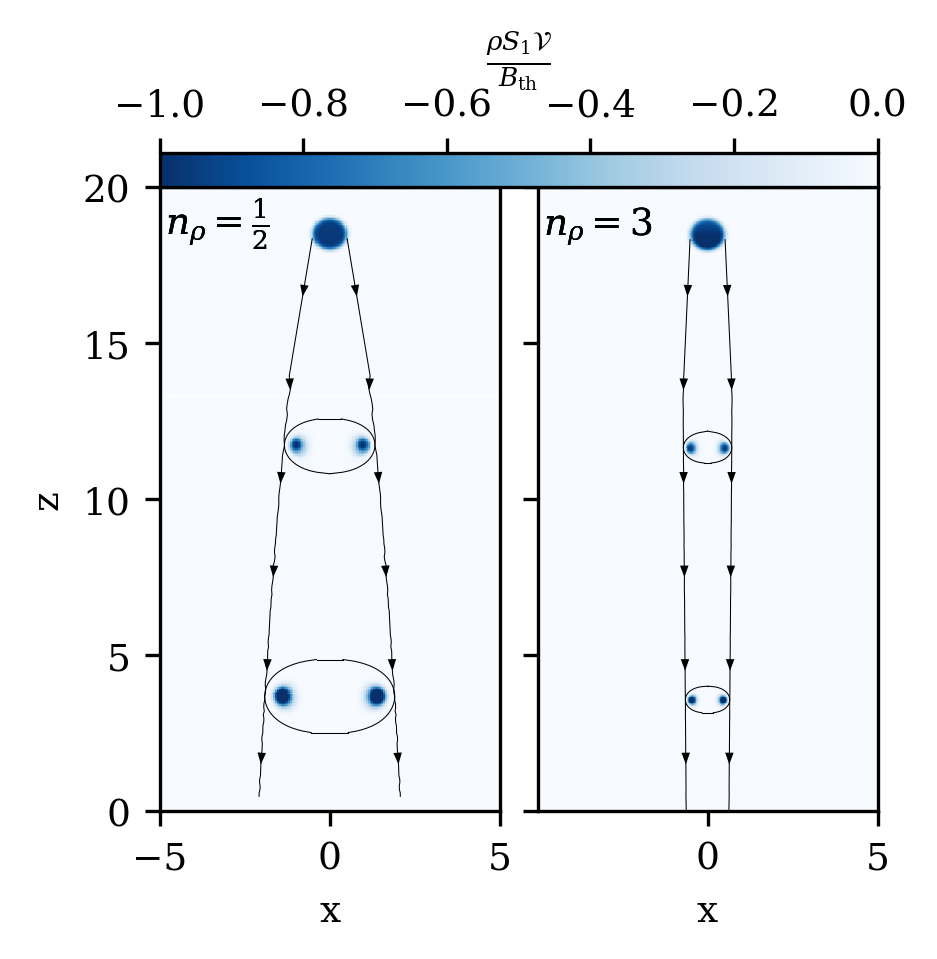
\includegraphics[width=\columnwidth]{evolution_colormeshes.png}
    \caption{The evolution of $\rho S_1 r^3$, or the total entropy weighted by
	the cube of the thermal radius, is shown for two thermals. On the left is
	a thermal in a weakly stratified domain with $n_\rho = 1/2$ density scale heights and 
	on the right is a thermal in a strongly stratified domain with $n_\rho = 3$.
	While both start with precisely the same initial condition, the case with low stratification
	expands with depth like the boussinesq case, whereas the strongly stratified thermal
	compresses with depth.
    \label{fig:evolution_colormeshes} }
\end{figure}


\subsection{Evolution of momentum and impulse}
The evolution of thermals as buoyant vortex rings has been well described in
the unstratified, Boussinesq limit for decades 
\citep[see e.g.][for a description and sources]{lecoanet&jeevanjee2018}.
Here we lay out a description of the momentum and
impulse of the thermal which will later be used 
to describe thermal properties like radii and depth vs. time.

In this work, we study an ideal gas and 
focus on the ideal, low Mach number regime in an adiabatically
stratified atmosphere. In this regime, a linearized equation of state describes
the thermodynamics well, and the fully compressible Euler momentum equation
takes the form \citep{brown&all2012},
\begin{equation}
\frac{\partial \bm{u}}{\partial t} + \bm{u}\cdot\grad\bm{u} = 
-\grad\varpi - \frac{S_1}{c_P}\bm{g},
\label{eqn:euler_momentum}
\end{equation}
where $\bm{u}$ is the velocity, $\varpi = P_1 / \rho_0$ is the reduced pressure,
$S = c_V\ln T - R\ln\rho$ is the specific entropy, and thermodynamics are broken
down into background (subscript 0) and fluctuating (subscript 1) components.
In this work we find it instructive to examine the full momentum, and so multiplying
this equation by the density, we obtain,
\begin{equation}
\frac{\partial (\rho\bm{u})}{\partial t} + \bm{u}\cdot\grad(\rho\bm{u}) + \rho\bm{u}(\DivU)
= -\rho\grad\varpi - \rho\frac{S_1}{c_P}\bm{g}.
\label{eqn:rho_euler_momentum}
\end{equation}
Hereafter we will define the Lagrangian derivative,
$D/Dt \equiv \partial/\partial t + \bm{u}\cdot\grad$, and we acknowledge that 
the Langrangian derivative commutes with a volume integral such that
\begin{equation*}
\frac{D}{Dt}\int_{\mathcal{V}} f dV = \int_{\mathcal{V}} \left[\frac{Df}{Dt} + f(\DivU)\right]dV.
\end{equation*}
Volume-integrating Eqn.~\ref{eqn:rho_euler_momentum}, we thus find
\begin{equation}
\frac{D\bm{M}}{Dt} = \int_{\mathcal{V}}\left(-\rho\grad\varpi - \rho\frac{S_1}{c_P}\bm{g}\right)dV,
\label{eqn:int_momentum_eqn}
\end{equation}
where the volume-integrated momentum is defined $\bm{M} \equiv \int_{\mathcal{V}}\rho\bm{u} dV$.
At this point we will make the assumption of a plane-parallel atmosphere in which the gravity
is constant, $\bm{g} = -g\hat{z}$, and note that the z-component of the volume-integrated
momentum evolves according to
\begin{equation}
\frac{D M_z}{Dt} = \int_{\mathcal{V}}\left( -\rho\frac{\partial \varpi}{\partial z} + \rho g \frac{S_1}{c_P} \right)dV.
\label{eqn:Mz_definition}
\end{equation}
At this point, we find it useful to define the total buoyancy,
\begin{equation}
B \equiv \int_{\mathcal{V}} \rho\, S_1\, \frac{g}{c_P}\, dV,
\label{eqn:tot_buoyancy}
\end{equation}
as in the absence of viscosity and detrainment, this is a conserved quantity during
thermal evolution (REFERENCE FIGURE). Furthermore, in the Boussinesq limit, the
work of \citet{tarshish&all2018} shows that pressure terms reduce the efficacy of
the buoyancy in changing the momentum by effectively reducing the buoyant acceleration
by some factor $\beta \sim 0.5$. As a result, we can approximate the growth of a thermal's
momentum according to
\begin{equation}
\frac{D M_z}{Dt} \approx \beta B.
\label{eqn:theory_momentum}
\end{equation}

After describing the growth of the thermal's integrated momentum with time, we turn
our attention to th ehydrodynamic impulse, which in the stratified limit is defined
\citep{shivamoggi2010},
\begin{equation}
\bm{I} = \frac{1}{2}\int_{\mathcal{V}} \bm{x}\times(\grad\times(\rho\bm{u}))dV,
\end{equation}
where $\bm{x}$ is the position vector. Impulse is equivalent to the time-integrated
work acting on the fluid resulting in the current fluid motion. 
Per \citet{shivamoggi2010}, changes in the impulse can be expressed as
\begin{equation*}
\frac{D\bm{I}}{D t} = \int_{\mathcal{V}}\frac{\partial(\rho\bm{u})}{\partial t}dV
= B\hat{z} - \int_{\mathcal{V}}\left[\rho\grad\varpi + \Div{\rho\bm{u}\bm{u}}\right]dV ,
\end{equation*}
where, importantly, the \emph{eulerian} derivative of the momentum is inside of the volume
integral here. Under the proper specification of boundary conditions, 
the integral term is zero, and the vertical impulse of a thermal thus straightforwardly
changes in time as
\begin{equation}
\frac{D I_z}{D t} = B.
\label{eqn:change_in_impulse}
\end{equation}
We have thus retrieved the two findings on which our theory of thermal evolution
will be built: \emph{both the impulse and momentum experience constant changes in
time determined by the buoyant nature of the thermal}.

\subsection{Parameterized description of thermal evolution}
\begin{figure}[t!]
    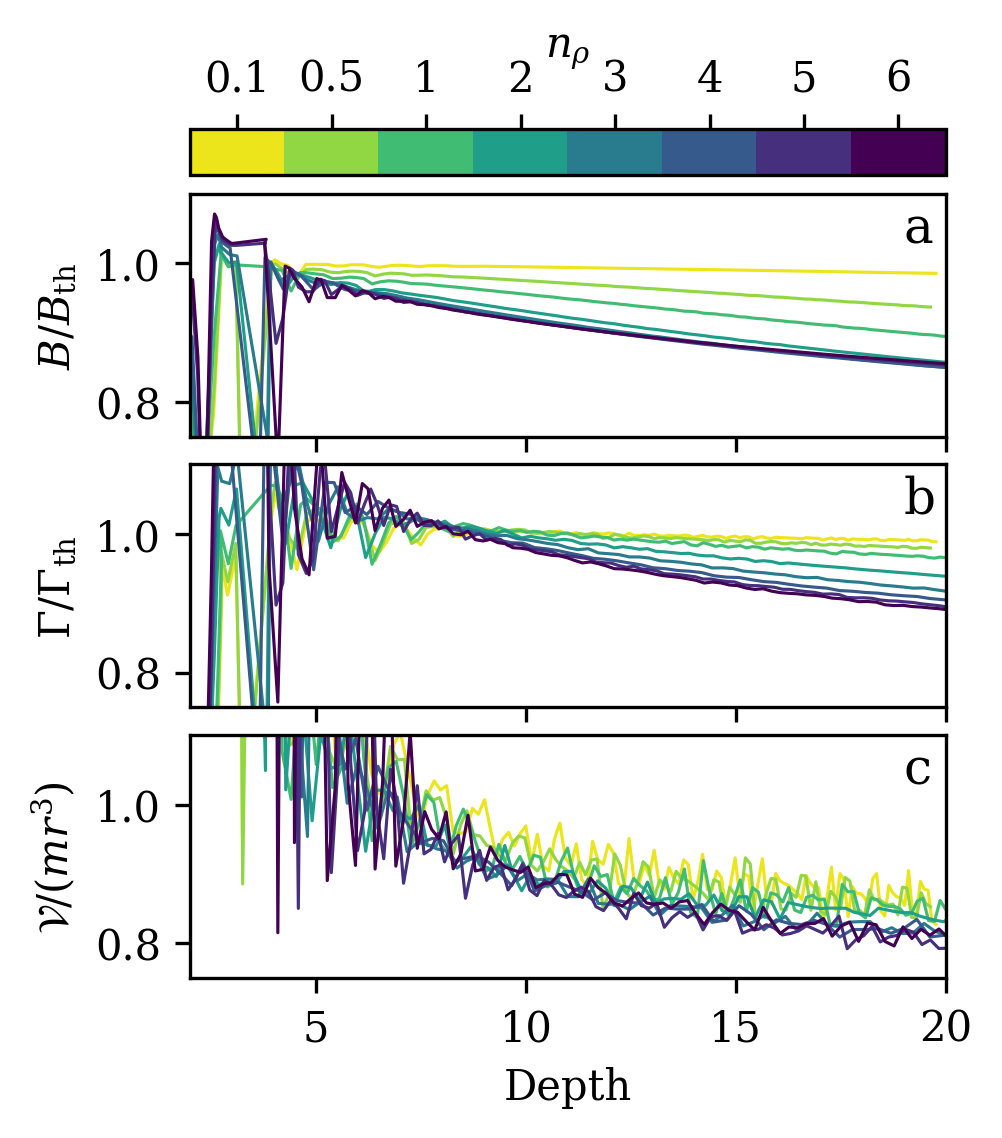
\includegraphics[width=\columnwidth]{constants.png}
    \caption{Plotted are time traces for three quantities which we assume to be constant
	in our thermal theory. In (a) and (b), the circulation and buoyancy, divided by their
	maxima, are plotted vs. depth. We see that with increasing stratification, there is marginally
	more detrainment of both of these quantities, but to first order they are constant over the
	evolution of the thermal. In (c) the constant $f = V/r^3$ is plotted; after significant
	noise during the development of the vortex ring, this quantity remains relatively constant, 
	and increasingly approaches a constant with depth.
    \label{fig:constants} }
\end{figure}



We first note, as in Fig.~\ref{fig:constants}a, that the buoyancy in our thermals
is not necessarily perfectly constant in time, and that effects like detrainment result
in a minor reduction of the buoyant signature of our thermals. We thus express the
buoyancy in terms of two constants,
\begin{equation}
B \approx \chi B_0,
\end{equation}
where $B_0$ is the initial buoyancy of the thermal, and $\chi$ is a constant of
O(1) which represents this detrainment. We then integrating 
Eqn.~\ref{eqn:change_in_impulse} in time,
\begin{equation*}
I_z = \chi B_0 t + I_0.
\end{equation*}
In the low-Mach number limit in which changes in density from the background are negligible,
the impulse of a vortex ring can be approximated as
\begin{equation*}
I_z \approx \pi \rho r^2 \Gamma_0,
\end{equation*}
where $r$ is the radius of the thermal from its axis
of symmetry to the maxima of its buoyant signature, and
$\Gamma_0 = \int_{\mathcal{A}} (\grad\times\bm{u})dA$ is the integrated circulation
in a cross-section of the vortex ring. We take $\Gamma_0$ to be constant, which is
a decent assumption in our experiments, see Fig.~\ref{fig:constants}b.
Combining these two expressions, we retrieve our first result,
\begin{equation}
r = \sqrt{\frac{\chi B_0 t + I_0}{\pi\rho\Gamma_0}}.
\label{eqn:r_theory}
\end{equation}
In the Boussinesq limit where $\rho \rightarrow \text{constant}$, 
we retrieve the $r \propto \sqrt{t}$ scaling found in the Boussinesq regime by
\citet{lecoanet&jeevanjee2018}. We find that the inclusion of stratification adds the
additional complexity of $r \propto \rho^{-1/2}$, such that downward-propogating 
vortex rings (as studied here) will entrain less than boussinesq thermals,
and upward-propogating rings will entrain more. In the absence of buoyancy ($B = 0$),
this result aligns with the prediction for purely horizontal compression noted by
\citet{brandenburg2016} of $r^2 \propto \rho^{-1}$.

The momentum can likewise be integrated like the impulse,
\begin{equation*}
M_z = \beta\chi B_0 t + M_0.
\end{equation*}
For the proper choice of vertical velocity, $w_{\text{th}}$, and volume, $\mathcal{V}$, the
momentum can be expressed precisely as 
\begin{equation*}
M_z = \rho \mathcal{V} w_{\text{th}},
\end{equation*}
and the volume can be approximated as $\mathcal{V} = f r^3$, where $f$ is a parameter
which we take to be constant. This assumption is perhaps not as perfect as the
assumptions of constant $B_0$ or $\Gamma_0$ (see Fig.~\ref{fig:constants}c), but
it is nevertheless not a bad assumption. Combining our approximate expressions,
and inserting our theoretical description of $r$ (Eqn.~\ref{eqn:r_theory}),
we retrieve
\begin{equation}
\rho^{-1/2} w_{\text{th}} = \left(\frac{(\pi \Gamma)^{3/2}}{f}\right)\frac{\beta\chi B_0 t + M_0}{(\chi B_0 t + I_0)^{3/2}}.
\end{equation}
Defining the thermal velocity $w_{\text{th}} \equiv dz_{\text{th}}/dt$, and making the
assumption that the vortex ring starts at a ``virtual origin'' (CITE) at $t = 0$ where
it has no impulse or momentum ($I_0 = M_0 = 0$), an integrable expression for the evolution
of thermal position over time can be retrieved,
\begin{equation}
\frac{dz_{\text{th}}}{\rho(z_{\text{th}})^{1/2}} =
\left(\frac{\beta(\pi\Gamma)^{3/2}}{f(\chi B_0)^{1/2}}\right)\frac{dt}{t^{1/2}}
\label{eqn:dz_theory}
\end{equation}
If the atmospheric stratification in which the thermal is falling is known, this
result can be integrated with $\rho(z_{\text{th}})$ plugged in in order to
find the position of the thermal as a function of time. We leave this result
general for now, and will integrate it using the polytropic stratification used in
our simulations at the end of section \ref{sec:experiment}.


%%%%%%%%%%%%%%%%%%%%%%%%%%%%%%%%%%%%%%%%%%%%%%%%%%%%%%%%%%%%%%%%%%%%%%%%%%%%%%%
%% EXPERIMENT SECTION
\section{Experiment} 
\label{sec:experiment}


\subsection{Anelastic Simulations}
In this work, we primarily study the evolution of 2D, azimuthally symmetric, anelastic
thermals in cylindrical coordinates. 
We later verify that select simulations produce the same results as 3D fully compressible
simulations in cartesian domains (see sec. REF). 
The LBR anelastic equations are \citep{lecoanet&all2014},
\begin{gather}
\td{\grad}\cdot\td{\bm{u}} = -\td{w}\partial_{\tilde{z}} \ln\rho_0 
\label{eqn:AN_continuity_full}\\
\frac{D \td{\bm{u}}}{D \td{t}} = -\td{\grad} \td{\varpi} + g\frac{\td{S_1}}{c_P}\hat{z} + \frac{1}{\rho_0}\td{\grad}\cdot\left(\mu\td{\lilstressT}\right)
\label{eqn:AN_momentum_full}\\
\frac{D \td{S_1}}{D\td{t}} = \frac{1}{\rho c_P}\td{\grad}\cdot\left(\kappa T_0 \td{\grad} \td{S_1}\right) + \frac{\mu}{\rho_0 T_0}\td{\sigma_{ij}}\partial_{\td{x_i}}\td{u_j}
\label{eqn:AN_energy_full}.
\end{gather}
where terms with tildes are dimensional, and where
$D/D\td{t} = \partial/\partial \td{t} + \td{\bm{u}}\cdot\td{\grad}$. In our azimuthally symetric
domain, we assume that $\partial_\phi = 0$; as the initial conditions of our simulations are at rest and have
no azimuthal velocity, $u_\phi$, we explicitly impose that $u_\phi = 0$; therefore $\bm{u} = u_r \hat{r} + w\hat{z}$. 
Under this approximation, the components of the stress tensor are
\begin{equation}
\begin{split}
&\td{\sigma}_{rr} = 2\frac{\partial \td{u_r}}{\partial \td{r}} - \frac{2}{3}\td{\grad}\cdot\td{\bm{u}},\,\,\,\,\,\,
\td{\sigma}_{\phi\phi} = 2\frac{\td{u_r}}{\td{r}} - \frac{2}{3}\td{\grad}\cdot\td{\bm{u}}, \\
&\td{\sigma}_{zz}       = 2\frac{\partial \td{w}}{\partial \td{z}} - \frac{2}{3}\td{\grad}\cdot\td{\bm{u}},\,\,\,\,\,\,\,
\td{\sigma}_{rz}     = \td{\sigma}_{zr} = \frac{\partial \td{w}}{\partial \td{r}} + \frac{\partial \td{u_r}}{\partial \td{z}}, \\
&\td{\sigma}_{r\phi}  = \td{\sigma}_{\phi r}  
 = \td{\sigma}_{\phi z} = \td{\sigma}_{z \phi}  = 0,\qquad
\end{split}
\end{equation}
Furthermore, we assume that the dynamic viscosity, $\mu = \rho_0 \nu$, and the
thermal conductivity, $\kappa = \rho_0 \chi$, are both uniform throughout the domain and
constant in time.
The diffusivities $\nu$ and $\chi$ therefore scale inversely with the density.

We nondimensionalize these equations in the same manner as in
\citet{lecoanet&jeevanjee2018} such that
the length scale is the diameter of the initial thermal perturbation
and the velocity scale is the freefall velocity. The timescale is thus
the freefall crossing time of this unit length. Mathematically,
\begin{equation}
\begin{split}
\td{\grad}\rightarrow(\td{L}_{th}^{-1})\grad, \qquad&
\td{S}_1 \rightarrow(\Delta\td{S})S_1,\\
\td{\bm{u}} \rightarrow (\td{u}_{th})\bm{u}, \qquad&
\td{\varpi} \rightarrow (\td{u}_{th}^2)\varpi,\\
\partial_{\tilde{t}} \rightarrow (\td{u}_{th}/\td{L}_{th})\partial_t,\qquad&
\end{split}
\end{equation}
with
\begin{equation}
\tilde{u}_{th}^2 = \frac{g \tilde{L}_{th} \Delta \tilde{s}}{c_P}, \qquad
\text{Re}_{\text{ff}} = \frac{\tilde{u}_{th} \tilde{L}_{th}}{\nu}, \qquad
\text{Pr}_{\text{ff}} = \frac{\tilde{u}_{th} \tilde{L}_{th}}{\chi}.
\end{equation}
As the diffusivities scale with depth, Re$_{\text{ff}}$ is specified at the
thermal's initial depth.
The resulting equations are,
\begin{gather}
\DivU = -w \partial_z \ln\rho_0, \\
\begin{split}
\partial_t \bm{u} + \bm{u}\cdot\grad&\bm{u} = \\
- \grad \varpi + S_1\hat{z} &
+ \frac{1}{\text{Re}_{\text{ff}}}\left[\grad^2 \bm{u} + \frac{1}{3}\grad(\DivU)\right] 
\end{split}\\
\begin{split}
\partial_t S_1 + \bm{u}\cdot\grad S_1 =& \\
\frac{1}{\text{Re}_{\text{ff}}}\left(\frac{1}{\text{Pr}_{\text{ff}}\rho_0c_P }\right.&[\grad^2 S_1 + \partial_z\ln T_0 \cdot\partial_z S_1]\\
&+ \left.\frac{-(\grad_{\text{ad}})}{\rho_0 T_0}\sigma_{ij}\partial_{x_i}u_j \right),
\end{split}
\end{gather}
where $\grad_{\text{ad}} \equiv \tilde{L}_{\text{th}} \frac{g}{c_P}$. 

\subsection{Atmosphere \& Initial conditions}
We study an ideal gas whose equation of state is $P = \rho T$ and whose stratification
is a perfectly adiabatic polytrope,
\begin{gather}
T_0 = 1 + (\grad_{\text{ad}})(z - L_z) \\
\rho_0 = T_0^{\,m_{\text{ad}}},
\label{eqn:polytrope}
\end{gather}
where $m_{\text{ad}} = (\gamma-1)^{-1}$, and the adiabatic temperature 
gradient in these nondimensional atmospheres is set with $g = m_{\text{ad}} + 1$
and $\tilde{L}_{\text{th}} = (e^{n_\rho/m_{\text{ad}}} - 1)/L_z$, where
$n_\rho$ is the number of density scale heights spanned by the atmosphere
and $L_z = 20$ is the nondimensional depth of the atmosphere in units of
thermal diameters.
 
To initialize the simulation, we specify a spherical initial specific entropy perturbation,
\begin{equation}
S_1 = - \frac{A}{2}\left[1 - \text{erf}\left(\frac{r' - r_{th}}{\delta}\right)\right],
\label{eqn:thermal_IC}
\end{equation}
where $A = 1$ for our scaled equations.
Here, $r' = \sqrt{r^2 + (z - z_0)^2}$, where $z_0 = L_z - 3r_{\text{th}}$,
with the thermal radius set as $r_{th} = 0.5$, and a smoothing width, $\delta = 0.1$.

\subsection{Fully Compressible Simulations}
In order to verify the validity of our 2D Anelastic simulations, we evolve select
thermals according to the 3D Navier Stokes equations in a cartesian domain. We use
the $(T, \ln\rho)$ formulation of the equations in which we have previously studied fully compressible
convection at low and high Mach number \citep{lecoanet&all2014, anders&brown2017},
\begin{gather}
\frac{D \ln\rho}{Dt} + \DivU = 0 \\
\frac{D \bm{u}}{D t} = -\grad T - T\grad\ln\rho - g\hat{z} + \frac{1}{\rho}\grad\cdot\left(\mu\lilstressT\right) \\
\frac{D T}{Dt} + (\gamma-1)T\DivU  = \frac{1}{\rho c_V}\grad\cdot\left(\kappa \grad T\right) + \frac{\mu}{\rho c_V}\sigma_{ij}\partial_{x_i}u_j.
\end{gather}
where the viscous stress tensor is defined as
\begin{equation}
\sigma_{ij} = \left(\partial_{x_i}u_j + \partial_{x_j}u_i - \frac{2}{3}\delta_{ij}\grad\cdot\bm{u}\right).
\end{equation}
These equations are nondimensionalized on the temperature gradient length scale such that
$\grad_{\text{ad}} = -1$ and the nondimensional timescale is the sound crossing time of that
unit length at the top of the domain.  

In setting the specific entropy, $S = c_V \ln T - R^{-1}\ln\rho$, to an equivalent condition
to that specified in  Eqn.~\ref{eqn:thermal_IC}, we note that it is essential that the
initial perturbation be in pressure equilibrium. The set of initial conditions that achieves this
is
\begin{equation}
\ln\rho_1 = S_1/c_P, \qquad T_1 = T_0(e^{-\ln\rho_1} - 1).
\end{equation}
We specify the magnitude of the initial entropy perturbations as 
$A = \epsilon = 10^{-4}$, such that the mach number of the resultant thermal is O($10^{-2}$) or less.

The depth of the atmosphere in these fully compressible domains is set to $L_z = e^{n_\rho/m_{ad}} - 1$.
In order to compare results from these
simulations to our Anelastic thermal simulations, we rescale all outputs in post-processing
by a length scale factor of $\ell = 20/L_z$, a timescales factor of  $\tau = \sqrt{\ell \epsilon}$,
and a specific entropy scaling of $s = \epsilon^{-1}$.

\subsection{Numerics}
We evolve our simulations forward in time using the 
Dedalus\footnote{\url{http://dedalus-project.org/}} 
pseudospectral framework \citep{burns&all2016} to time-evolve
our equations. For our 2D simulations, we use 
using an implicit-explicit (IMEX), third-order, four-stage
Runge-Kutta timestepping scheme RK443 \citep{ascher&all1997},
and for our 3D simulations we use the second order
semi-implicit backward differentiation formulation
SBDF2 \citep{wang&ruuth2008}.

Our 3D simulations are decomponsed on Fourier bases in the horizontal
directions ($x, y \in [-L_r, L_r]$) and Chebyshev bases vertically
($z \in [0, L_z]$) with impenetrable, stress free, fixed-temperature
boundary conditions at the upper and lower boundaries 
($T_1 = w = \partial_z u = \partial_z v = 0$ at $z = [0, L_z]$).
Our 2D simulations are decomposed on a Fourier $(z \in [0, L_z])$ and
Chebyshev $(r \in [0, L_r])$ domain, with boundary conditions of
$\partial_r S_1 = w = (\grad\times\bm{u})_{\phi} = 0$ at $r = L_r$.


\subsection{Solution for thermal evolution in a Polytrope}
Now that the atmospheric density is specific, we can 
find an explicit solution for Eqn.~\ref{eqn:dz_theory} to compare
to the results of our simulations. As temperature and height are
linearly related in our atmospheres, we find it instructive to use
temperature as a integration parameter.
We note that, $\rho = T^{m_{ad}}$ and
$dT = (\grad_{\text{ad}}) dz_{th}$, such that we must solve
\begin{equation}
\int_{T_0}^{T_{\text{th}}} T^{-m_{ad}/2} dT 
= \left(\frac{\beta(\pi\Gamma)^{3/2}\grad_{\text{ad}}}{f(\chi B)^{1/2}}\right)
\int_{0}^{t + t_{\text{off}}} t^{-1/2} dt.
\end{equation}
defining $C \equiv \beta \pi^{3/2} \grad_{\text{ad}} / f \sqrt{\Gamma^3/(\chi B)}$
and $\alpha^{-1} = 1 - m_{\text{ad}}/2$, and 
ssuming that $m_{\text{ad}} < 2$ (which is valid for our case of $m_{\text{ad}} = 1.5$
studied here) we find that
\begin{equation}
T_{\text{th}} = \left(\frac{2C}{ \alpha } \sqrt{t + t_{\text{off}}} + T_0^{1/\alpha}  \right)^{\alpha}.
\label{eqn:theory_T}
\end{equation}
In the limit of large stratification, we thus find that $T_{\text{th}} \propto t^2$ for
our case of $\alpha = 4$. The temperature can be straightforwardly converted to height
by a rearrangement of Eqn.~\ref{eqn:polytrope},
\begin{equation}
z_{\text{th}} = (T_{\text{th}} - 1)/\grad_{\text{ad}} + L_z
\end{equation}
The thermal is thus described in terms of seven total parameters:
\begin{enumerate}
\item $T_0$ and $t_{\text{off}}$, the temperature of the thermal's virtual origin, and
the time before the simulation's $t = 0$ at which the thermal was located at its virtual origin,
\item $B_0$ and $\Gamma$, the measurable buoyancy and circulation of the vortex ring, and
\item $f$, $\chi$, and $\beta$, fitting parameters which describe the nature of the vortex
ring's evolution.
\end{enumerate}
The measured values of these parameters for the cases studied in this paper are presented
in table \ref{table:parameters}.

\begin{deluxetable*}{c c c c c c c c c}
\tabletypesize{\footnotesize}
\caption{Simulation output parameterization
\label{table:parameters}
}
\tablehead{																																															
\colhead{$n_\rho$} & \colhead{$\grad_{\text{ad}}$} & \colhead{$T_0$} & \colhead{$t_{\text{off}}$} & \colhead{$B$} & \colhead{$\Gamma$} & \colhead{$f$} & \colhead{$\chi$} & \colhead{$\beta$}	}	
\startdata																																															
\multicolumn{9}{l}{\textbf{2D Anelastic Simulations}}\\
0.1 	& $3.45 \times 10^{-3}$		& 0.985	& 0.166	& -0.547 & -2.17 & 7.01	& 1.04	& 0.499	\\
0.5 	& $1.98 \times 10^{-2}$		& 0.918	& 0.704	& -0.568 & -2.12 & 7.04	& 0.976	& 0.490	\\
1	 	& $4.74 \times 10^{-2}$		& 0.827	& 1.09 	& -0.601 & -2.05 & 7.07	& 0.915	& 0.480	\\
2	 	& $0.140$             		& 0.677	& 1.26	& -0.712 & -1.89 & 7.08	& 0.841 & 0.456	\\
3	 	& $0.319$             		& 0.619	& 1.01	& -0.946 & -1.73 & 7.08	& 0.808	& 0.436	\\
4	 	& $0.667$             		& 0.698	& 0.622	& -1.47	 & -1.59 & 7.10	& 0.793	& 0.422	\\
5	 	& $1.352$             		&			& 			&	 &	&	&	&	\\
\multicolumn{9}{l}{\textbf{3D Fully Compressible Simulations}}\\    
0.5 	& 	$1.98 \times 10^{-2}$	& 0.924	& 0.583	& -0.568 & -2.12 & 6.66	& 0.978	& 0.452	\\
1	 	& 	$4.74 \times 10^{-2}$	& 0.832	& 1.26	& -0.601 & -2.05 & 6.88	& 0.902	& 0.454	\\
2	 	& 	$0.140$             	& 0.666	& 1.53	& -0.711 & -1.89 & 7.08	& 0.822	& 0.450	\\
\enddata																																															
\tablecomments{ Values from fully compressible simulations have been rescaled
in post-processing for direct comparison with 2D anelastic cases}
\end{deluxetable*}




%%%%%%%%%%%%%%%%%%%%%%%%%%%%%%%%%%%%%%%%%%%%%%%%%%%%%%%%%%%%%%%%%%%%%%%%%%%%%%%
%% RESULTS SECTION
\section{Results}
\label{sec:results}

\begin{figure}[t!]
    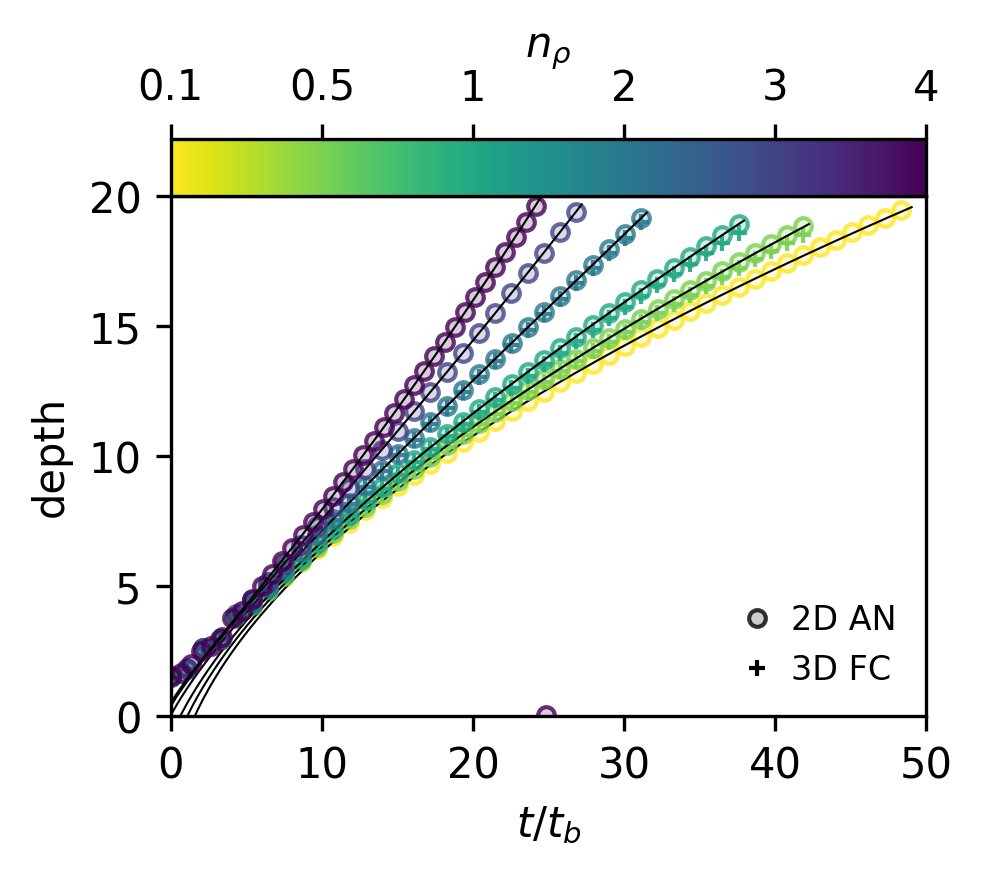
\includegraphics[width=\columnwidth]{results_panels_d_v_t.png}
    \caption{Shown are the measured depths of thermals as a function of time for all 2D
	Anelastic and 3D Fully compressible simulations conducted in this work. Overplotted
	is the theoretical prediction for depth as a function of time.
    \label{fig:results_d_v_t} }
\end{figure}

\begin{figure}[t!]
    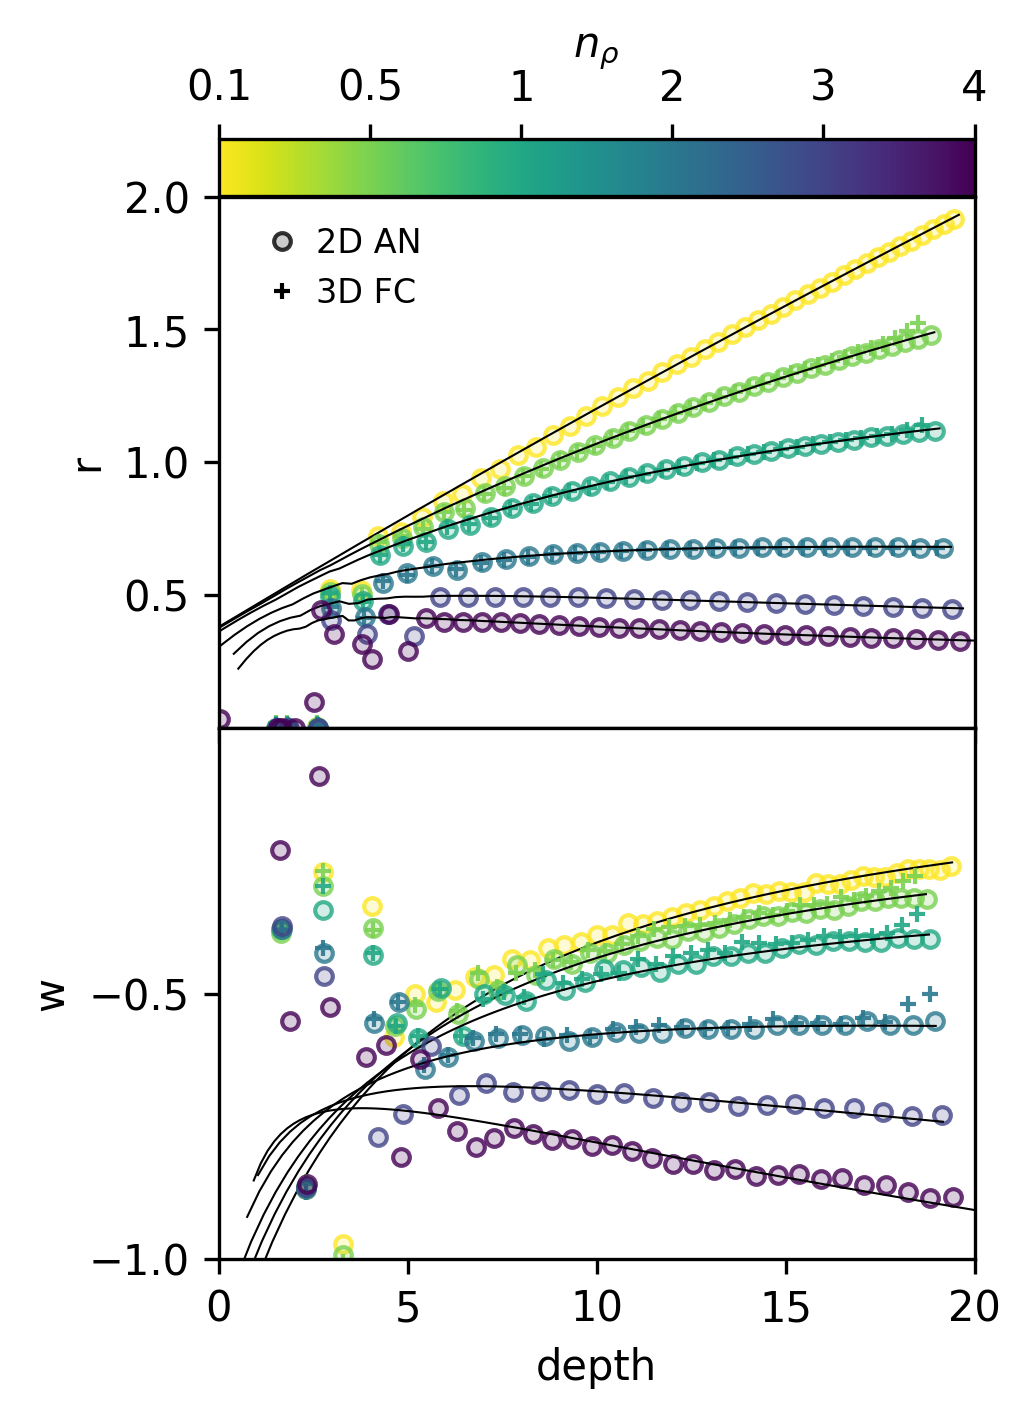
\includegraphics[width=\columnwidth]{results_panels_vs_depth.png}
    \caption{Shown are (a) the measured radii of thermals as a function of depth and
	(b) the measured thermal velocities as a function of depth for all 2D
	Anelastic and 3D Fully compressible simulations conducted in this work. Overplotted
	are the predictions from theory.
    \label{fig:results_vs_depth} }
\end{figure}

In Fig. \ref{fig:results_d_v_t}, we show the measured depth $d_{\text{th}} = L_z - z_{\text{th}}$
of the thermal as a function of time for low and high stratification. 
At very low stratification
(e.g., $n_\rho = 0.1$), the thermal is small compared to the local density scale height at all depths,
and it evolves roughly according to the Boussinesq prediction of $d \propto \sqrt{t}$. As the stratification
increases, 
the thermal begins to transit the domain more quickly and approaches the limit of 
$d \propto t^2$ predicted in the highly stratified limit of Eqn.~\ref{eqn:theory_T}. The
theoretical fits for depth from the prediction of Eqn.~\ref{eqn:theory_T} are plotted over
the measured data and show remarkable agreement.

In Fig.~\ref{fig:results_vs_depth}a, we plot the measured thermal radius vs. depth, with the
theoretical predictions of Eqns.~\ref{eqn:r_theory} \& \ref{eqn:theory_T} plotted as lines
over the data. In the low stratification limit, the radius of the thermal grows linearly with
depth, $r \propto d$, aligning with the Boussinesq limit shown in \citet{lecoanet&jeevanjee2018} 
This growth of the thermal is the result of entrainment of environmental fluid and
results an an accompany decceleration like $w \propto d^{-1}$ in the Boussinesq limit, 
as is shown in Fig.~\ref{fig:results_vs_depth}b.
However, as stratification increases, the thermal entrains less environmental fluid and
expands less, eventually even contracting with depth in the high-stratification limit. 
This lessened entrainment is, unsurprisingly, accompanied by greater acceleration of the thermal.
As in the case of depth vs. time, the overplotted theoretical predictions show excellent
agreement with the measured data.

These results suggest that there are two regimes of downflowing thermal behavior:
\begin{enumerate}
\item A low-stratification ``stalling'' regime, in which the thermal entrains environmental
fluid and slows down, acting much like the Boussinesq regime, and
\item A high-stratification ``falling'' regime, in which the thermal falls fast enough
that compression due to the atmospheric stratification results in minimal entrainment and
the thermal accelerates as it falls deeper into the atmosphere.
\end{enumerate}
However, we note that both of these regimes could result in interesting problems for the
entropy rain hypothesis. If solar convection were comprised of thermals in the stalling regime,
it is unlikely that such elements would ever make it to the base of the solar convection zone, 
stalling much closer to the solar surface and depositing their entropy signature there -- possibly
agreeing with the hypothesis of supergranulation as the largest buoyantly driven scale of
solar motion. On the other hand, if solar convection is comprised of thermals in the falling
regime, then it is possible that as these thermals compress and accelerate, diffusive effects
and potentially viscous heating could become important. We discuss these possibilities further
in section \ref{sec:discussion}

\subsection{Verification of 2D Anelastic approximation}
\begin{figure*}[t!]
    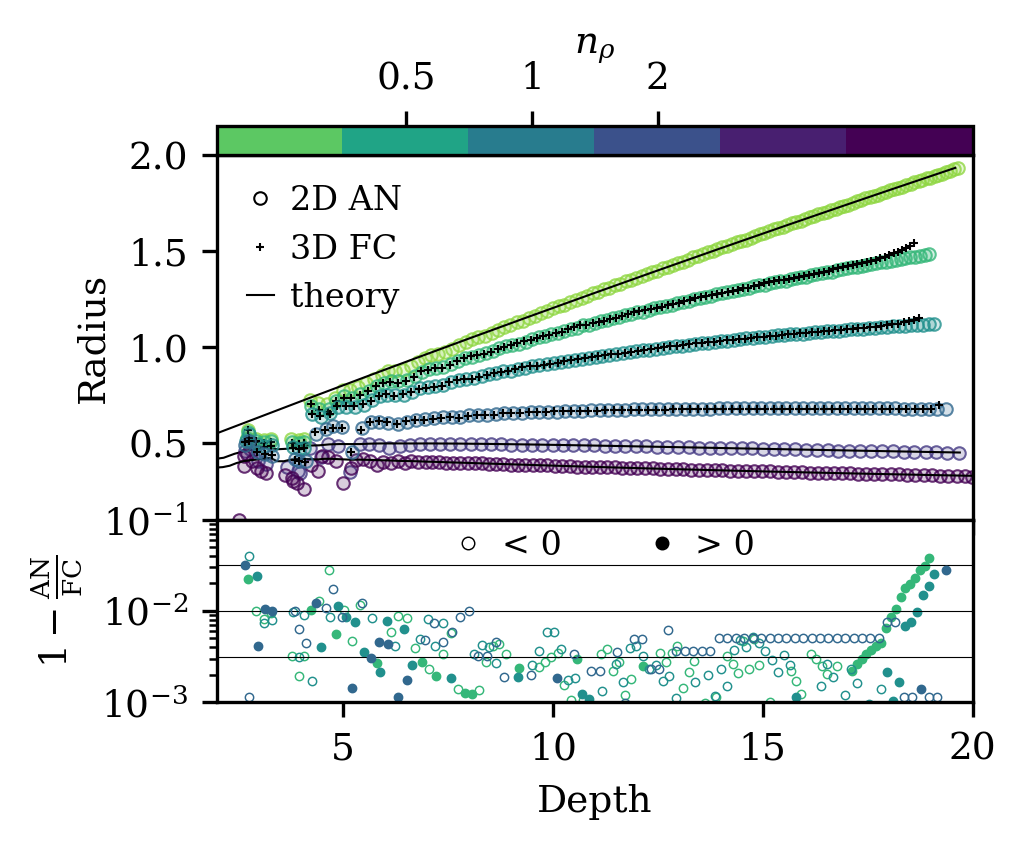
\includegraphics[width=\textwidth]{diff_AN_FC.png}
    \caption{Measured values of (a) depth vs. time and (c) radius vs. depth are plotted
	for both the 2D anelastic and 3D fully compressible simulations. The fractional
	difference between anelastic and fully compressible results are respectively shown
	in (b) and (d).
    \label{fig:diff} }
\end{figure*}

In Fig.~\ref{fig:diff}, we display in more detail a comparison of our 2D Anelastic and
3D Fully Compressible cases. In Fig.~\ref{fig:diff}a, depth vs time is shown, and the
fractional difference between FC and AN cases is shown in Fig.~\ref{fig:diff}b.
Differences between the two cases are $\leq 2$\% for all times, with greater error towards
the end of the simulations as the FC simulations begin to interact with the impenetrable
boundary at the bottom of their simulation domains.  In Fig.~\ref{fig:diff}c, radius
vs. depth is shown, and the fractional difference between FC and AN cases is shown in
Fig.~\ref{fig:diff}d. Aside from the very end of the simulation when the FC boundary conditions
begin to matter, there is remarkable agreement between the two cases, with $< 1$\% differences
between the two cases after early times in which the thermal is still developing into a vortex
ring.

This close agreement between low Mach number Fully Compressible simulations and Anelastic
simulations parallels the agreement between the equation sets seen in \citet{lecoanet&all2014},
and gives us confidence in our anelastic results at higher levels of stratification, where
the 2D simulations are much more numerically feasible than the 3D fully compressible simulations.


%%%%%%%%%%%%%%%%%%%%%%%%%%%%%%%%%%%%%%%%%%%%%%%%%%%%%%%%%%%%%%%%%%%%%%%%%%%%%%%
%% CONCLUSION SECTION
\section{Discussion}
\label{sec:discussion}
In this work we have extended the theory of the evolution of buoyant thermals into the
low-Mach number, stratified regime and have shown that that theory has remarkable agreement
with the results of both Anelastic and Fully compressible simulations.

We should have some discussion on these topics:
\begin{enumerate}
\item speculation about extensions to the solar regime. Do things on the sun shrink
to the point where they viscously dissipate? Do they stall?
\item Talk about what would happen if we were to study up-thermals.
\item Extensions, and we trust that these results should hold in the regime of solar convection
where things are turbulent.
\end{enumerate}

\begin{acknowledgements}
This work was supported by NASA Headquarters under the NASA Earth and Space
Science Fellowship Program -- Grant 80NSSC18K1199.
This work was additionally supported by  NASA LWS grant number NNX16AC92G.  
Computations were conducted 
with support by the NASA High End Computing (HEC) Program through the NASA 
Advanced Supercomputing (NAS) Division at Ames Research Center on Pleiades
with allocation GID s1647.
\end{acknowledgements}

\appendix
\section{Thermal Tracking}
\label{appendix:tracking}
We use a thermal tracking algorithm very similar to the one used in 
\citet{lecoanet&jeevanjee2018} and inspired by the work of 
\citet{romps&all2015}. 

We begin by measuring the thermal's height versus
time. To do so, we average the domain's entropy profile in radius and azimuth
to create an average profile of entropy with height, and then assume that the
thermal's vortex core is located at the entropy minima of each of those profiles.
We numerically differentiate these found values of height vs. time using
(insert numerical differentiation technique here) and then calculate the streamfunction of
the velocity field as in \citet{romps&all2015},
\begin{equation}
\frac{\partial \psi}{\partial r} = 2\pi \rho r (w - w_{\text{th}}),
\end{equation}
with the boundary condition that $\psi = 0$ at $r = 0$. The contour defined by $\psi = 0$
from this solution is taken to be the outline of the thermal, and the volume of the thermal
is taken to be the volume radially inward from that contour.


\section{Table of Simulations}
\label{appendix:table}

\begin{deluxetable*}{c c c c c c}
\tabletypesize{\footnotesize}
\caption{Table of simulation information
\label{table:simulation_info}
}
\tablehead{																																															
\colhead{$n_\rho$} & \colhead{$L_r$} & \colhead{nr or nx = ny} & \colhead{nz} & \colhead{$t_{evolution}$} & \colhead{safety}	}	
\startdata																																															
\multicolumn{6}{l}{\textbf{2D Anelastic Simulations}}\\
0.1 	& 	7				&	512			& 512			& 49 	&	0.1	\\
0.5 	& 	7				&	512			& 512			& 42.5 	&	0.1	\\
1	 	& 	5				&	512			& 512			& 38 	&	0.1	\\
2	 	& 	5				&	512			& 512			& 31.75	&	0.1	\\
3	 	& 	5				&	1024		& 1024			& 27.25	&	0.1	\\
4	 	& 	5				&	1024		& 1024			& 25 	&	0.075	\\
5	 	& 	2.4				&	1024		& 1024			& 22.8 	&	0.05	\\
\multicolumn{6}{l}{\textbf{3D Fully Compressible Simulations}}\\
0.5 	& 	5				&	256			& 512			& 42.5 		&	0.8	\\
1	 	& 	4				&	256			& 512			& 38 	 	&	0.8	\\
2	 	& 	3.5				&	256			& 1536			& 31.75 	&	0.8	\\
\enddata																																															
\tablecomments{
}
\end{deluxetable*}

\bibliography{../tex/biblio.bib}

\listofchanges
\end{document}
